\documentclass[11pt]{scrartcl}
\usepackage[sexy]{evan}
\usepackage{graphicx}
\graphicspath{ {./images/} }

\usepackage{answers}
\Newassociation{hint}{hintitem}{all-hints}
\renewcommand{\solutionextension}{out}
\renewenvironment{hintitem}[1]{\item[\bfseries #1.]}{}

\usepackage{venndiagram,multicol,hyperref,graphicx,array}

\begin{document}
\title{Conteo I}
\author{Ricardo Largaespada}
\date{17 Febrero 2024}

\maketitle

\section{Introducción}

¿Cuántas formas podemos vestirnos? ¿Y cuántos números menores que 1000 tienen todas las cifras pares? Contar cosas es una actividad tan antigua como la propia humanidad. Desde los primeros tiempos, los seres humanos han buscado formas de organizar y cuantificar su entorno.

Sin embargo, con el transcurso del tiempo, nuestras técnicas para contar y resolver problemas matemáticos han evolucionado significativamente. Han surgido nuevas herramientas y métodos que nos permiten abordar problemas de manera más eficiente y sistemática.

Aunque la forma más básica de contar es hacerlo caso por caso, esta estrategia puede resultar tediosa y poco práctica en situaciones más complejas. Es aquí donde entran en juego técnicas más avanzadas de conteo, que nos permiten resolver problemas de manera más eficiente y elegante.

En esta clase, exploraremos algunas de estas técnicas y cómo pueden aplicarse a una amplia gama de problemas. A través de ejemplos y ejercicios prácticos, aprenderemos a utilizar herramientas como el principio de multiplicación, el principio de adición, la combinatoria y otras estrategias para abordar problemas de conteo de manera más sofisticada y efectiva. Comencemos explorando estas técnicas con un ejemplo concreto:

\section{Problemas Resueltos}
\begin{example}
Una puerta se abre cuando utilizamos simultáneamente la llave y la tarjeta correctas. Si tenemos dos llaves y tres tarjetas, ¿cuántas pruebas debemos hacer para garantizar que la puerta se abrirá?
\end{example}
Podemos elaborar un diagrama (\ref{fig_1}) que nos ayude a resolver el problema.

\begin{figure}
    \centering
    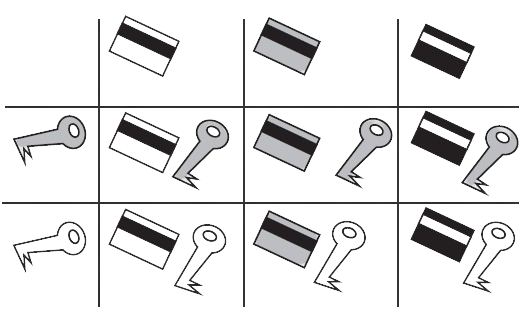
\includegraphics[scale=.25]{clase_04_llaves_tarjeta.png}
    \caption{Figura}
    \label{fig_1}
\end{figure}

En el diagrama anterior podemos ver todas las combinaciones posibles de una llave y una tarjeta. Por lo tanto, la solución es visual e igual a 6. Por otra parte, podríamos haber resuelto el problema de la siguiente manera:\\

Observa que para cada elección de llave hay tres formas de elegir la tarjeta. Como tenemos dos llaves, el número total de combinaciones es 2 × 3 = 6. En este caso, harían falta 6 pruebas para encontrar la combinación correcta.\\

Así, si hubiera 30 llaves y 5 cartas, no sería necesario hacer un diagrama para contar las combinaciones una a una, el resultado sería simplemente $30 \times 5 = 150$. El método que acabamos de utilizar se conoce como \textit{principio multiplicativo}. En los próximos problemas lo utilizaremos de forma más general.

\begin{example}
Teddy tiene 5 blusas, 3 pares de pantalones y 2 pares de zapatos. ¿De cuántas maneras diferentes puede vestirse?
\end{example}

Contemos primero el número de maneras en que Teddy puede elegir su camisa y sus pantalones. Pues bien, por cada par de pantalones que Teddy elija, tiene cinco maneras más de elegir su blusa. Como tiene tres pantalones, el número total de maneras de elegir el par (pantalón y blusa) es $5 \times 3 = 15$. Ahora bien, por cada forma de elegir este par, le quedan dos formas de elegir los zapatos. Por lo tanto, es fácil concluir que Teddy puede vestirse de $5 \times 3 \times 2 = 30$ maneras diferentes.

\begin{example}
¿De cuántas maneras podemos pintar un tablero de 1 × 4 utilizando sólo tres colores, sin pintar los cuadrados vecinos del mismo color?\\
\begin{tabular}{|c|c|c|c|}
\hline
 & & & \\
\hline
\end{tabular}
\end{example}

Podemos pintar el primer cuadrado de tres formas distintas, el segundo de dos formas distintas (no podemos utilizar el color del primer cuadrado), el tercer cuadrado se puede pintar de dos formas distintas (no podemos utilizar el color del segundo cuadrado), y lo mismo ocurre con el cuarto cuadrado. Así que el número total de formas de colorear el tablero es $3 \times 2 \times 2 \times 2 = 24$.\\

Supongamos que Carlos, Felipe, Marina y Ana están en fila. Si cambiamos la posición de alguno de ellos, decimos que hemos hecho una \textit{permutación}. La pregunta es: ¿Cuántas permutaciones podemos tener utilizando cuatro personas? Antes de resolver el problema, vamos a introducir una notación que se utiliza a menudo en problemas de recuento porque simplifica algunos cálculos.

\begin{claim}
    Dado un número natural \( n \), sea \( n! \) (léase \( n \) factorial) el producto \( 1 \times 2 \times 3 \times \ldots \times (n-1) \times n \).
\end{claim}

Obsérvese que el concepto de factorial está fuertemente ligado a la noción de permutación. Para consolidar esta notación, resolvamos algunos ejercicios sencillos:
\begin{enumerate}
    \item Calcula \(4!, 5!\) y \(6!\).
    \item Calcular \(\displaystyle\frac{100!}{98!}\) y \(\displaystyle\frac{47!}{44!3!}\).
    \item Resuelve la ecuación \((m + 2)! = 72 \cdot m!\).
    \item Probar que \begin{enumerate}
        \item \(\displaystyle \frac{1}{n!}-\frac{1}{(n+1)!}=\frac{n}{(n+1)!}\)
        \item \(2\cdot 4\cdot 6\cdots (2n)=2^n\cdot n!\)
    \end{enumerate}
\end{enumerate}

\begin{example}
¿De cuántas formas podemos formar una cola con Carlos, Felipe, Marina y Ana?
\end{example}

Podemos elegir al primero de la cola de cuatro maneras, al segundo de tres, al tercero de dos y al último de una sola manera (la persona que queda). De este modo tenemos \(4 \times 3 \times 2 \times 1 = 4!\) permutaciones.

\begin{example}
En un reloj digital, la hora se muestra con cuatro dígitos. El reloj cambia de 00:00 a 23:00. ¿Cuántas veces al día se muestran los cuatro dígitos pares?
\end{example}

Observa que en este problema hay una restricción sobre los dígitos que marcan las horas y el primer dígito que marca los minutos. Así que en lugar de pensar en cada dígito por separado, pensemos en tres bloques de dígitos. El primero, que está formado por los dos primeros dígitos, puede tomar 7 valores diferentes (00, 02, 04, 06, 08, 20 ó 22); el segundo está formado sólo por el tercer dígito y puede tomar 3 valores (0, 2 ó 4); y el último dígito puede tomar 5 valores (0, 2, 4, 6 u 8). Por lo tanto, el número total de veces que aparecen todos por parejas es \(7 \times 3 \times 5 = 105\).\\

Preocupémonos ahora de algunos problemas más ``clásicos''. Aunque estos problemas son bien conocidos por todos, los trataremos aquí porque emplean ideas que se utilizan constantemente en diversos problemas.

\begin{example}[Número de subconjuntos]
¿Cuántos subconjuntos tiene el conjunto \( M = \{1, 2, 3, \ldots, 10\} \)?
\end{example}

A cada subconjunto de \( M \) asociaremos una secuencia de 10 dígitos que pueden ser 0 ó 1. Esta asociación vendrá dada por la siguiente regla: El primer término de esta secuencia será 1 si el elemento 1 está en el subconjunto y 0 en caso contrario; El segundo término de esta secuencia será 1 si el elemento 2 está en el subconjunto y 0 en caso contrario; El tercer término de esta secuencia será 1 si el elemento 3 está en el subconjunto y 0 en caso contrario; y así sucesivamente.\\

Por ejemplo, el subconjunto \(\{1, 2, 5, 8, 10\}\) está asociado a la secuencia \(1100100101\), el subconjunto \(\{2, 3, 5, 8\}\) está asociado a la secuencia \(0110100100\), mientras que el subconjunto vacío \(\{\emptyset\}\) está representado por \(0000000000\). Obsérvese que el número de subconjuntos de \( M \) es igual al número de estas secuencias. Por otra parte, podemos elegir cada dígito de dos maneras y, en consecuencia, tenemos \(2^{10}\) secuencias (que es el mismo número de subconjuntos).

\begin{example}[Número de divisores]
Sea \( n = p_1^{\alpha_1}p_2^{\alpha_2}\cdots p_k^{\alpha_k} \) un número natural en su forma factorizada. Entonces \( n \) tiene exactamente \[ (\alpha_1 + 1)(\alpha_2 + 1) \cdots (\alpha_k + 1) \] divisores enteros positivos, incluyendo \(1\) y \(n\).
\end{example}

Tenga en cuenta que cada divisor positivo de \( n \) es de la forma \( p_1^{\beta_1}p_2^{\beta_2}\cdots p_k^{\beta_k} \), donde cada exponente \( \beta_i \) es un número entre 0 y \( \alpha_i \) (inclusive). Así, tenemos \( (\alpha_1 + 1) \) formas de elegir el exponente de \( p_1 \); \( (\alpha_2 + 1) \) formas de elegir el exponente de \( p_2 \); y así sucesivamente. Así que el resultado del principio multiplicativo sigue.

\Opensolutionfile{all-hints}

\section{Problemas Propuestos}
\begin{problem}
En una habitación hay 3 hombres y 4 mujeres. ¿De cuántas maneras es posible
seleccionar una pareja?
\begin{hint}
    .
\end{hint}
\end{problem}

\begin{problem}
Cada casilla de un tablero de 2×2 puede ser de color verde o amarillo. ¿De cuántas formas podemos colorear todo el tablero?
\begin{hint}
    .
    \end{hint}
\end{problem}

\begin{problem}[OBM 2004]
¿De cuántas formas diferentes podemos pintar (utilizando un solo color) los cuadrados de un tablero de \(4 \times 4\) de manera que en cada fila y columna haya exactamente un cuadrado pintado?
    \begin{hint}
    .
    \end{hint}
\end{problem}

\begin{problem}
¿Cuántos números naturales hay con tres cifras distintas?
\begin{hint}
.
\end{hint}
\end{problem}

\begin{problem}
¿De cuántas maneras podemos colocar tres torres de tres colores diferentes en un tablero de $8 \times 8$ de forma que ninguna de ellas ataque a otra?
    \begin{hint}
    .
    \end{hint}
\end{problem}

\begin{problem}
Una barca debe estar tripulada por ocho hombres, dos de los cuales reman a la derecha y uno sólo a la izquierda. Determina de cuántas maneras se puede formar esta tripulación si hay cuatro hombres en cada lado. Nota: Hay que tener en cuenta el orden de los hombres.
    \begin{hint}
    .
    \end{hint}
\end{problem}

\begin{problem}
¿De cuántas maneras podemos ir de A a B en la siguiente cuadrícula sin pasar dos veces por el mismo sitio y sin movernos a la izquierda? La figura siguiente muestra un camino posible.
\begin{center}
    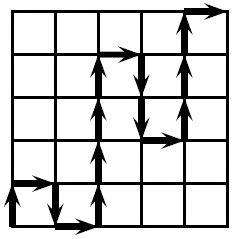
\includegraphics[scale=0.4]{clase_04_camino.png}
\end{center}
    \begin{hint}
    .
    \end{hint}
\end{problem}

\begin{problem}
Halla el número de números de cuatro cifras tales que cada secuencia de tres cifras consecutivas está formada por elementos distintos.
\begin{hint}
    .
\end{hint}
\end{problem}

\begin{problem}[OBM 2005]
En un tablero cuadrado de $5 \times 5$, se colocarán tres botones idénticos, cada uno en el centro de un cuadrado, formando un triángulo. ¿De cuántas maneras podemos colocar los botones para formar un triángulo rectángulo de lados paralelos?
\begin{hint}
    .
\end{hint}
\end{problem}

\begin{problem}
Decimos que la palabra algoritmo es un anagrama de la palabra logaritmo porque es una permutación de las letras logaritmo. Sabiendo esto, calcula el número de anagramas de la palabra vector.
\begin{hint}
    .
\end{hint}
\end{problem}

\begin{problem}
¿Cuántos anagramas de la palabra vector terminan en vocal?
\begin{hint}
    .
\end{hint}
\end{problem}

\begin{problem}
¿De cuántas maneras puedes colocar 5 libros de matemáticas, 3 de física y 2 de biología en una estantería para que los libros de la misma asignatura permanezcan juntos?
\begin{hint}
    .
\end{hint}
\end{problem}

\begin{problem}
¿Cuántos anagramas de la palabra vector tienen vocales separadas?
\begin{hint}
    .
\end{hint}
\end{problem}

\begin{problem}
¿De cuántas maneras podemos colocar 4 bolas verdes y 4 amarillas en un tablero de \(4 \times 4\) de forma que en cada columna y fila haya exactamente una bola de cada color?
\begin{hint}
    .
\end{hint}
\end{problem}

\begin{problem}
Contesta a las siguientes preguntas:
\begin{enumerate}[a)]
    \item Halla el número de divisores positivos de 3600.
    \item ¿Cuántos de estos divisores son pares?
    \item ¿Cuántos son cuadrados perfectos?
\end{enumerate}
\begin{hint}
    .
\end{hint}
\end{problem}
\begin{problem}[Olimpiada de Mayo 2006]
Un calendario digital muestra la fecha: día, mes y año, con 2 dígitos para el día, 2 dígitos para el mes y 2 dígitos para el año. Por ejemplo, 01-01-01 corresponde al 1 de enero de 2001 y 25-05-23 corresponde al 25 de mayo de 2023. Delante del calendario hay un espejo. Los dígitos del calendario son como los de la imagen de abajo.
\begin{center}
    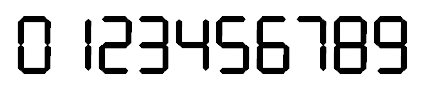
\includegraphics[scale=0.5]{clase_04_mayo.png}
\end{center}
Si 0, 1, 2, 5 y 8 se reflejan respectivamente en 0, 1, 5, 2 y 8, y los demás dígitos pierden su significado al reflejarse, determina cuántos días del siglo, al reflejarse en el espejo, corresponden también a una fecha.
\begin{hint}
    .
\end{hint}
\end{problem}

\begin{problem}[Rusia]
    Se dice que un número natural \(n\) es \textit{elegante} si se puede escribir como la suma de un cubo y un cuadrado (\( n = a^3 + b^2 \), donde \( a, b \in \mathbb{N} \)). Entre 1 y 1000000, ¿hay más números que sean elegantes o que no lo sean?
\begin{hint}
    .
\end{hint}
\end{problem}

\begin{problem}
¿Cuántos números de cinco cifras son múltiplos de 3 y tienen 6 como una de sus cifras?
\begin{hint}
    .
\end{hint}    
\end{problem}
\Closesolutionfile{all-hints}

\begin{comment}
\section{Sugerencias}
\begin{enumerate}
\input{all-hints.out}
\end{enumerate}
\end{comment}

\end{document}